\chapter{Usability Evaluation}
\label{chapter:Usability}

To ensure the \ac{splash} system aligns with user needs and expectations, a usability evaluation was conducted during the Construction phase using low-fidelity prototypes, as described in Chapter~\ref{chapter:Mockups}. This evaluation aimed to identify usability issues early and to guide design decisions for the subsequent development stages.

\section{Methods}

\subsection{Wizard of Oz Approach}
The Wizard of Oz technique was employed to simulate system functionalities without full implementation. During testing, participants interacted with interfaces as though they were functional, while the underlying responses were manually controlled by a facilitator. This method enabled the team to evaluate user behavior and expectations in a realistic yet controlled manner.

\subsection{Usability Testing Procedure}

\begin{itemize}
    \item \textbf{Participants:} Five users participated in the usability evaluation. They were selected to represent the primary personas defined in Chapter4\ref{chapter:UserCenteredDesign}, including lifeguard supervisors, regular lifeguards, beachgoers, and business owners.
    
    \item \textbf{Tasks:} Participants were asked to complete scenario-based tasks derived from their respective personas, such as locating lifeguard stations, signaling hazards, managing schedules, and requesting assistance. These tasks were grounded in real use cases identified during the requirements and task analysis stages.

    \item \textbf{Think-Aloud Protocol:} Participants were encouraged to verbalize their thoughts while performing tasks, allowing the facilitators to gain insights into user expectations, reasoning processes, and usability challenges.

    \item \textbf{Observation and Note-Taking:} The research team recorded user interactions, behavioral patterns, and errors during testing sessions, supported by photographs (e.g., Figure~\ref{fig:usability-testing}).

    \item \textbf{Post-Test Feedback:} Following the tasks, participants provided qualitative feedback through brief interviews and completed a System Usability Scale (SUS) questionnaire to quantify the overall usability of the prototype.
\end{itemize}

All participants signed an informed consent document before the evaluation and were informed that they could stop the session at any time without justification.

\section{Evaluation Objective}
The primary goal of this evaluation was to validate whether the SPLASH prototype could achieve a SUS score of at least 70, a widely accepted threshold for acceptable usability in interactive systems. This metric was also defined as a success criterion for the project.

\section{Results and Insights}

The average SUS  score obtained across all participants was \textbf{77.5}(see Figure~\ref{fig:sus_score}), meeting the defined usability goal. The evaluation also revealed the following:

\begin{itemize}
    \item \textbf{Strengths:} Participants praised the clarity of the interactive map, the perceived usefulness of hazard alerts, and the logical task flows for reporting and requesting assistance.

    \item \textbf{Usability Issues:} Some users experienced initial confusion when accessing the schedule management features and interpreting certain map symbols.

    \item \textbf{Suggestions:} Users suggested visual improvements (e.g., color contrast), more explicit icons for dangerous areas, and tooltips for new users unfamiliar with the interface.

    \item \textbf{General Feedback:} Participants reported a high level of satisfaction with the system's potential impact on beach safety, particularly the real-time information and GPS bracelet integration.
\end{itemize}
\begin{figure}[H]
    \centering
    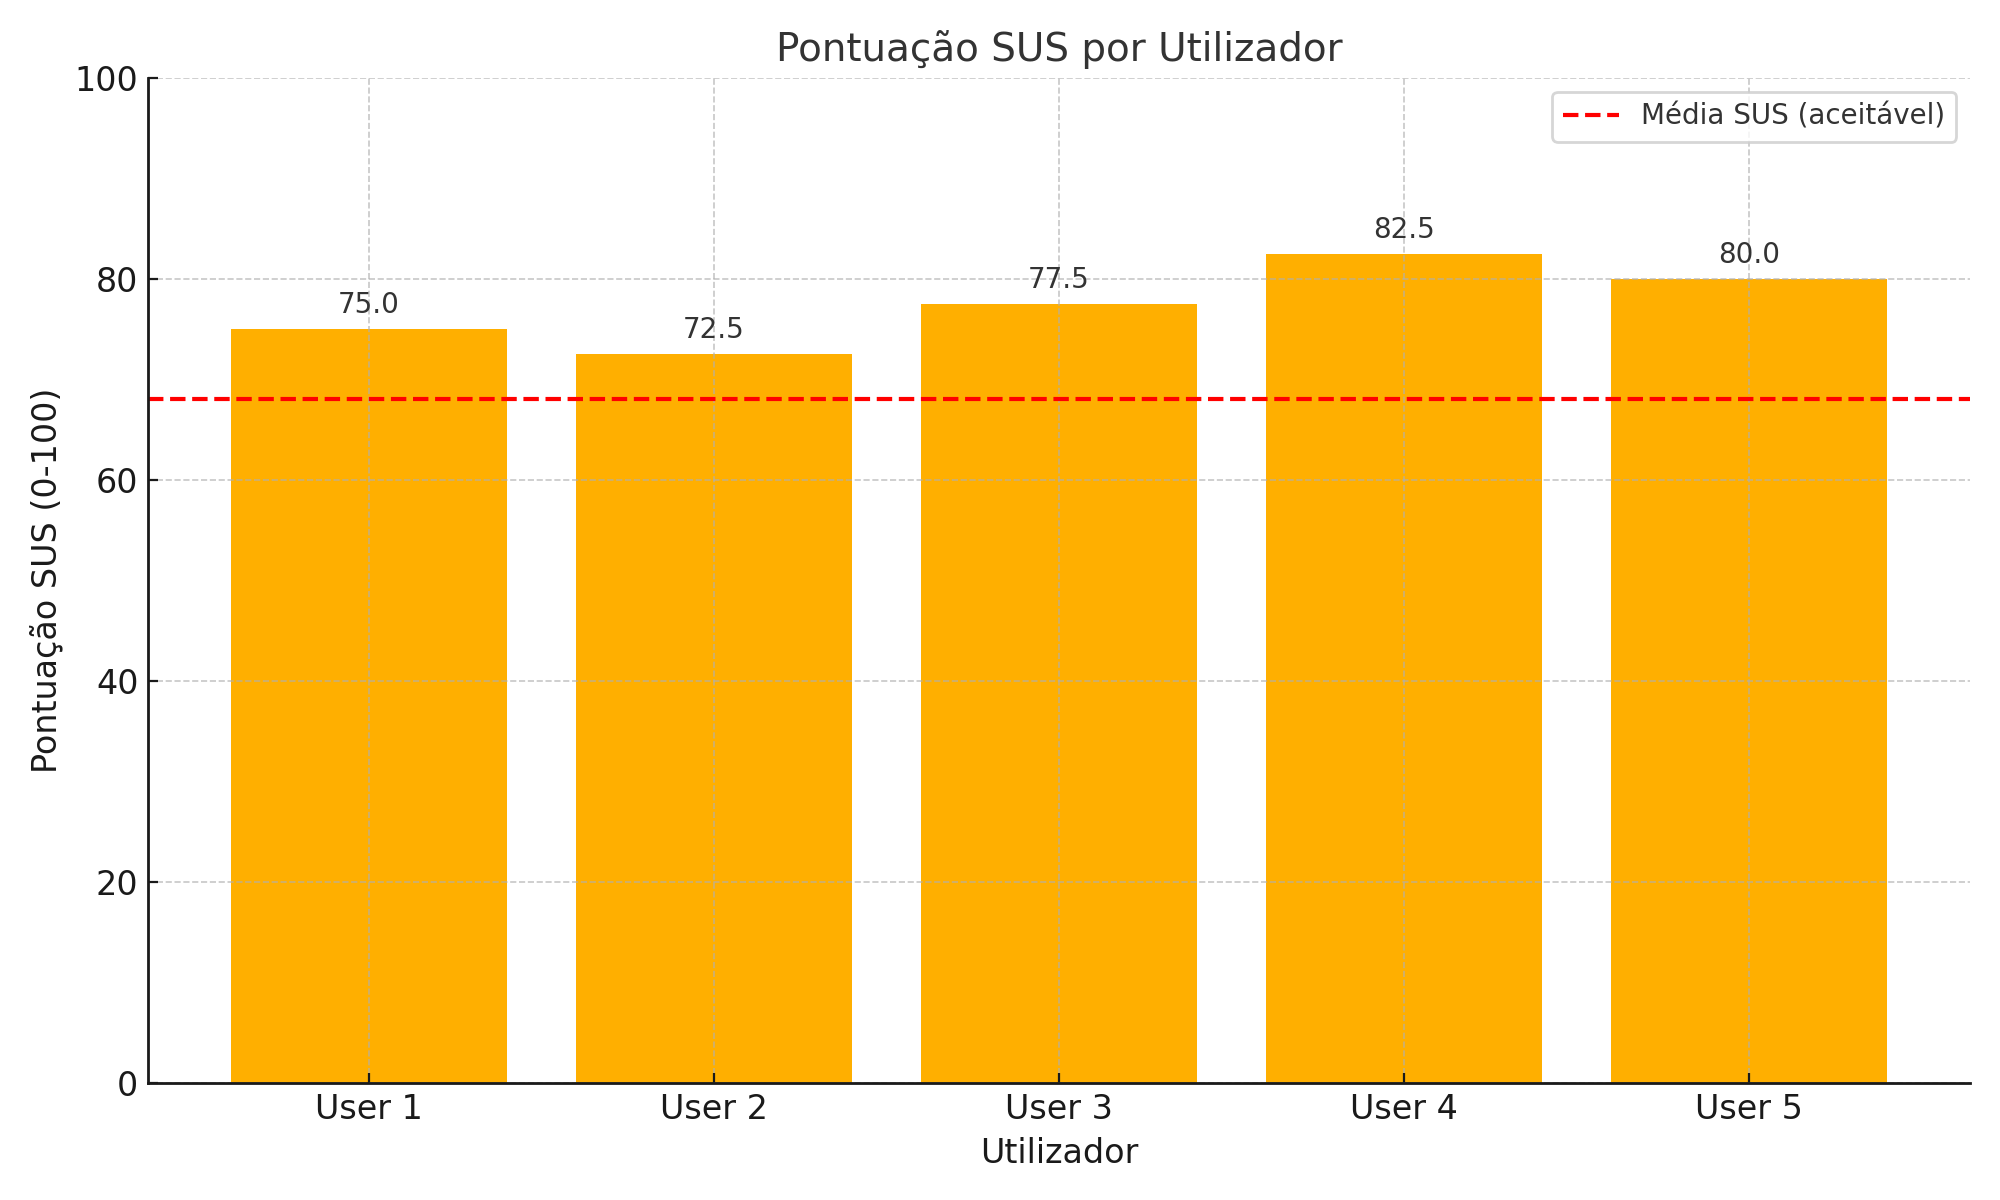
\includegraphics[width=13cm,height=10cm]{figs/SUS_Poster_Grafico.png}
    \caption{\ac{splash}: SUS score}
    \label{fig:sus_score}
\end{figure}
\section{Summary}
The usability evaluation provided critical insights into the prototype’s effectiveness, revealing both its strengths and improvement areas. The methodology, combining the Wizard of Oz technique with structured testing, proved successful in simulating real-world interactions. The SPLASH system met its usability benchmark, supporting its viability as a user-centered digital solution for coastal safety management.

\begin{figure}[H]
    \centering
    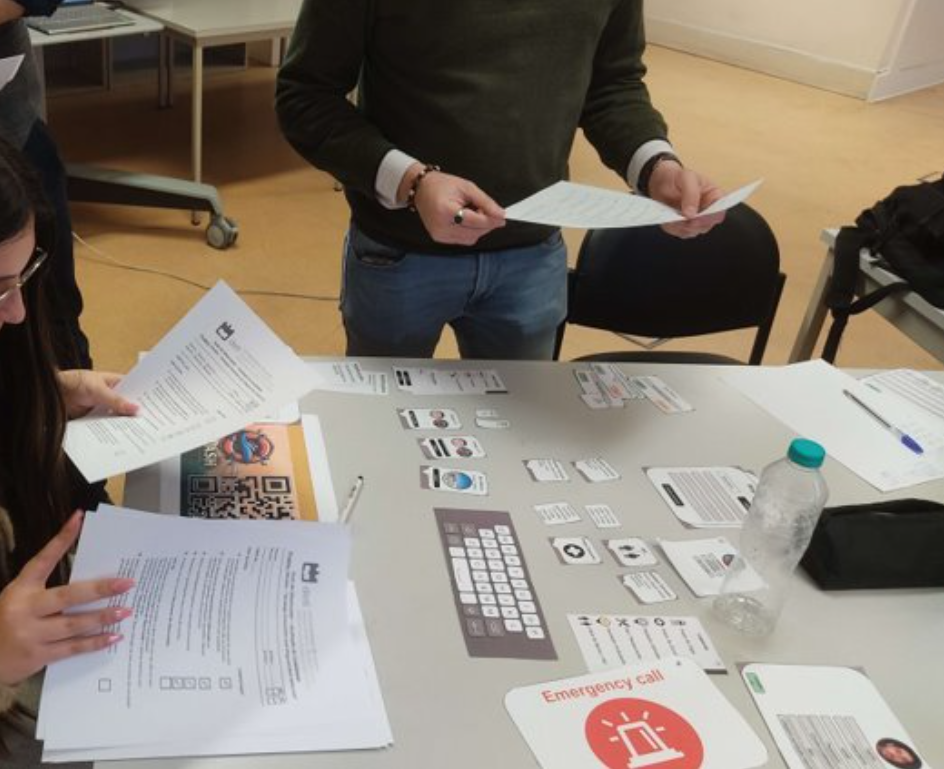
\includegraphics[width=13cm,height=10cm]{figs/mockup-tests.png}
    \caption{\ac{splash}: Photograph captured during a usability testing session with users}
    \label{fig:usability-testing}
\end{figure}
